\chapter{Capacitación y Concientización}
\label{ch:capacitacion_concientizacion}

\section{Enfoque Estratégico y Factor Humano en la UNAP}

El eslabón humano representa históricamente la superficie más explotada en las instituciones de educación superior. Los relevamientos pasivos ejecutados sobre el dominio \texttt{unap.edu.pe} confirmaron debilidades críticas en la capa de mensajería (ausencia de directivas DMARC y política SPF con directiva permisiva \texttt{\textasciitilde all}), configurando un entorno propicio para ataques de ingeniería social orientados a la captura de credenciales académicas y administrativas.

El Programa Institucional de Capacitación y Concientización en Ciberseguridad de la Universidad Nacional del Altiplano de Puno trasciende la instrucción teórica pasiva. Su objetivo es instaurar una cultura de desconfianza positiva y verificación activa, transformando a los más de 20,000 miembros de la comunidad universitaria en la primera línea de detección temprana institucional (\textit{Firewall Humano}).

El programa articula tres (3) ejes formativos diferenciados y adaptados al perfil de riesgo:

\begin{center}
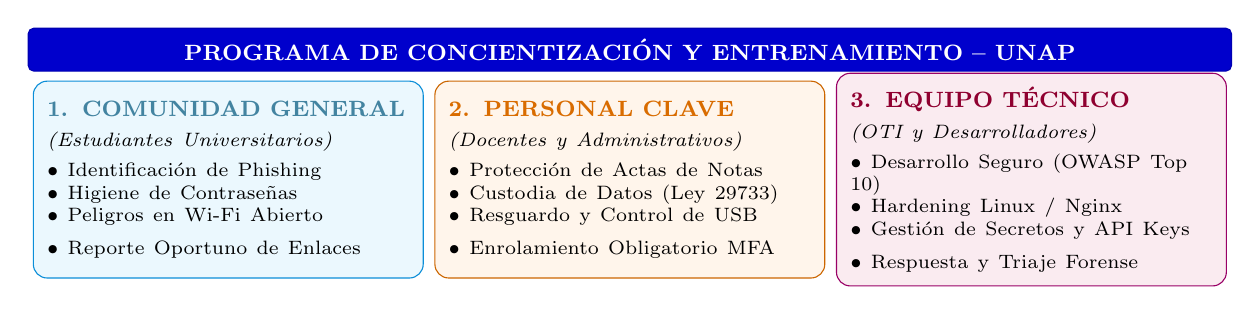
\begin{tikzpicture}[
    titleBar/.style={
        draw=blue!70!black, fill=blue!80!black, text=white,
        font=\bfseries\footnotesize, align=center,
        inner sep=4pt, text width=15.0cm, rounded corners=2pt
    },
    axisCard/.style={
        rectangle, rounded corners=5pt,
        inner sep=5pt, text width=4.6cm,
        minimum height=2.5cm, align=left
    }
]

\node[titleBar] (topBar) at (0, 0) {PROGRAMA DE CONCIENTIZACIÓN Y ENTRENAMIENTO -- UNAP};

% Eje 1: Comunidad General
\node[axisCard, draw=cyan!75!blue, fill=cyan!8] (c1) at (-5.1, -1.65) {
    {\bfseries\footnotesize\color{cyan!60!black} 1. COMUNIDAD GENERAL}\\[-1pt]
    {\scriptsize\itshape (Estudiantes Universitarios)}\\[3pt]
    \scriptsize
    $\bullet$ Identificación de Phishing\\
    $\bullet$ Higiene de Contraseñas\\
    $\bullet$ Peligros en Wi-Fi Abierto\\
    $\bullet$ Reporte Oportuno de Enlaces
};

% Eje 2: Personal Clave
\node[axisCard, draw=orange!80!black, fill=orange!8] (c2) at (0, -1.65) {
    {\bfseries\footnotesize\color{orange!85!black} 2. PERSONAL CLAVE}\\[-1pt]
    {\scriptsize\itshape (Docentes y Administrativos)}\\[3pt]
    \scriptsize
    $\bullet$ Protección de Actas de Notas\\
    $\bullet$ Custodia de Datos (Ley 29733)\\
    $\bullet$ Resguardo y Control de USB\\
    $\bullet$ Enrolamiento Obligatorio MFA
};

% Eje 3: Equipo Técnico
\node[axisCard, draw=purple!80!blue, fill=purple!8] (c3) at (5.1, -1.65) {
    {\bfseries\footnotesize\color{purple!75!black} 3. EQUIPO TÉCNICO}\\[-1pt]
    {\scriptsize\itshape (OTI y Desarrolladores)}\\[3pt]
    \scriptsize
    $\bullet$ Desarrollo Seguro (OWASP Top 10)\\
    $\bullet$ Hardening Linux / Nginx\\
    $\bullet$ Gestión de Secretos y API Keys\\
    $\bullet$ Respuesta y Triaje Forense
};

\end{tikzpicture}
\end{center}

\section{Módulos Temáticos de Capacitación Institucional}

El plan de estudios obligatorio para el personal administrativo y docente se estructura en los siguientes seis (6) módulos operacionales:

\begin{enumerate}[leftmargin=1.4em, itemsep=1.5pt, parsep=0.5pt, topsep=2pt]
    \item \textbf{Phishing e Ingeniería Social:} Reconocimiento de técnicas de persuasión psicológica, urgencia inducida y suplantación de identidad; verificación rigurosa de URLs en enlaces institucionales (diferenciando los portales legítimos \texttt{matri\allowbreak cula.\allowbreak unap.\allowbreak edu.pe} y \texttt{campus.\allowbreak unap.\allowbreak edu.pe} de dominios apócrifos y typosquatting); e inspección de discrepancias en cabeceras y nombres de remitente.
    
    \item \textbf{Higiene de Contraseñas y Adopción de MFA:} Creación de contraseñas de alta entropía (mínimo 12 caracteres alfanuméricos combinados con símbolos); erradicación terminante de contraseñas por defecto basadas en el número de DNI o códigos de matrícula; obligatoriedad en el uso de aplicaciones de segundo factor basadas en tiempo (TOTP) y concientización contra la fatiga de notificaciones push.
    
    \item \textbf{Protección de Datos Personales (Ley N° 29733):} Custodia de bancos de datos personales; prohibición estricta de compartir registros de notas, planillas o expedientes de estudiantes por canales no cifrados o redes sociales abiertas; y aplicación del principio de puesto de trabajo limpio y pantalla bloqueada.
    
    \item \textbf{Seguridad en Correo Electrónico y Navegación Web:} Identificación de archivos adjuntos potencialmente maliciosos camuflados como documentos PDF o actas de notas; verificación de navegación segura mediante HTTPS estricto; y prevención de riesgos al navegar en redes Wi-Fi abiertas sin conexión VPN institucional cifrada.
    
    \item \textbf{Riesgos de Almacenamiento Extraíble (USB):} Prevención de infecciones cruzadas por memorias USB desconocidas en laboratorios de cómputo y dependencias administrativas; protocolos de desinfección obligatoria y bloqueo preventivo de ejecución automática (\textit{AutoRun}).
    
    \item \textbf{Procedimiento de Notificación Rápida:} Entrenamiento práctico en el uso del botón institucional de reporte de phishing en el cliente de correo webmail y uso del canal directo con el CSIRT-UNAP (\texttt{seguridad.\allowbreak informatica@\allowbreak unap.\allowbreak edu.pe} / \texttt{csirt@\allowbreak unap.\allowbreak edu.pe}).
\end{enumerate}

\section{Metodología de Simulaciones de Phishing Controlado}

Para medir de forma empírica la vulnerabilidad del personal universitario y condicionar el reflejo de alerta temprana, la Oficina de Tecnologías de la Información (OTI) ejecutará campañas de simulación trimestrales sin preaviso, utilizando plataformas dedicadas de emulación de adversarios (GoPhish / Microsoft Defender Attack Simulation).

\subsection*{Fases de la Simulación Operativa}

\begin{itemize}[leftmargin=1.4em, itemsep=1.5pt, parsep=0.5pt, topsep=2pt]
    \item \textbf{Fase 1: Diseño de Vectores Contextuales.} Construcción de señuelos hiperrealistas alineados al calendario académico y administrativo de la UNAP (por ejemplo, falsos comunicados de \textit{Regularización urgente de notas}, \textit{Encuesta obligatoria de acreditación institucional}, o \textit{Nuevo cronograma de pagos de Tesorería}).
    
    \item \textbf{Fase 2: Lanzamiento Controlado.} Envío escalonado a subconjuntos aleatorios de cuentas de correo institucional (\texttt{@unap.edu.pe}) del personal administrativo, autoridades y docentes de las 20 facultades.
    
    \item \textbf{Fase 3: Registro y Análisis de Métricas de Interacción.} Registro automatizado y trazable de: correos entregados, correos abiertos, clics en el enlace malicioso simulado, credenciales ingresadas en la página trampa y reportes legítimos recibidos en el CSIRT institucional.
    
    \item \textbf{Fase 4: Retroalimentación Formativa Inmediata (\textit{Just-in-Time Training}).} Aquellos usuarios que introduzcan sus credenciales en el portal simulado serán redirigidos de inmediato a una página interactiva educativa que expone los indicadores de engaño que pasaron por alto, asignándoles automáticamente una microcápsula formativa obligatoria de 10 minutos.
\end{itemize}